\chapter{Effects of Pulse Amplitude and Pulse Rate Modulation during Acute Electrical Stimulation with a Vestibular Implant in Human Patients}\label{chap:pamprm}
\chaptermark{Effects of Pulse Modulation during Acute VI Stimulation}

\subparagraph{Abstract}
Patients instrumented with vestibular implants have shown preliminary encouraging results, but the different effects of stimulation strategies based on pulse rate (PRM) or pulse amplitude modulation (PAM) have not been yet identified. Here, we address this issue by acutely testing a vestibular implant in four bilateral vestibular loss subjects using either PAM or PRM. 

At a super-physiological baseline pulse rate, PAM evoked stronger eye movement responses than comparable PRM. Lowering the baseline pulse rate significantly reduced the PAM response, but did not significantly change the PRM response.

We also developed a neural network model that simulated the implant interacting with the vestibular nuclei and reproduced the relationships from the clinical tests. This model revealed that PAM consistently causes greater changes in recruitment and firing rate than PRM due to both the initial adaptation to implant activation, and the interdependency of stimulation parameters and afferent resting discharge rate. 

Our findings suggest PAM as the preferred strategy for initial activation in human vestibular implants. Chronic studies are necessary to reveal whether VOR plasticity can enhance the response to the vestibular implant. 

\section{Introduction}
The vestibular system plays an essential role in everyday life. Being at the interface of sensory and motor systems, it contributes to various levels of nervous function. For example, the vestibulo-ocular reflex (VOR) drives stabilization of gaze during head motion, while other pathways influence postural control and spatial orientation. All these rely on the input from the peripheral vestibular organs in the inner ear. When vestibular function is lost bilaterally, patients typically suffer for instance from imbalance, impaired spatial orientation, or oscillopsia. The prognosis of bilateral vestibular loss (BVL) is bleak (Zingler et al., 2008), patients have a reduced quality of life (Guinand et al., 2012) and no adequate treatment option is available.

Research in animal models have partially restored vestibular function (Merfeld and Lewis, 2012). Performance was typically quantified via the VOR response. Early experiments with patients demonstrated viability (Guyot et al., 2011a; Guyot et al., 2011b) and we recently reported single-axis VOR restoration (Perez Fornos et al., 2014) and VOR dependency on modulation frequency (Van De Berg et al., 2015). A vestibular implant (VI) could therefore prompt significant rehabilitation.

Prototypes in animal models have predominantly employed pulse rate modulation (PRM) to replicate primary afferents’ natural spike rate modulation (Fernandez and Goldberg, 1971). Pulse amplitude modulation (PAM) and co-modulation of pulse amplitude and pulse rate also evoked considerable eye movements (Davidovics et al., 2010; Davidovics et al., 2012). The conundrum whether PRM or PAM is more effective has recently gained relevance as modified cochlear implants, which effectively use PAM to transmit sound information, have become available for vestibular stimulation.

To address this issue, we tested four patients with VIs based on modified cochlear implants providing independent electrodes to stimulate vestibular nerve branches. We characterized their eye movement responses to PAM and PRM during acute trials. Specifically, we injected equal amounts of charge with both paradigms to compare their efficacies. To unify the experimental results, we built a simple, but biologically inspired model of VOR driven by electrical stimulation. The model was adapted only to continuous baseline stimulation present at implant activation. It then reproduced the relationships between PRM and PAM found in acute experiments and provided interesting insights about possible results of chronic stimulation. Our findings indicate PAM as preferential paradigm – at least during the acute stage after implant activation. 

\section{Methods}
\subsection{Patients}
Experiments were performed in accordance with the Declaration of Helsinki. The ethics committees of the University Hospitals Geneva (NAC 11-080) and the Maastricht University Medical Center (NL36777.068.11/METC 11-2-031) approved this study. 

Among a pool of eleven patients that received modified cochlear implants (MED-EL, Innsbruck, Austria), four patients were available for this study (named BVL1 – BVL4, Table\,\ref{tab:pamprm}). The stimulation sites were in proximity to the ampullae of the lateral, superior or posterior ampullary nerve (LAN, SAN and PAN, respectively). Details on inclusion criteria, implant and surgical approaches have been published elsewhere (Van De Berg et al., 2012; Perez Fornos et al., 2014).

\subsection{Stimulation and Recording Paradigm}
Patients were tested acutely, 2-3 hours per electrode, and remained seated in a non-moving chair in a dark room. Stimulation was controlled with a customized system (Nguyen et al., 2014). The baseline pulse amplitude was set approximately in the middle of the dynamic range, i.\,e., between lower (vestibular) and upper (comfortable) thresholds (Perez Fornos et al., 2014). Baseline stimulation was maintained for 30 minutes for all vestibular symptoms such as nystagmus to subside (Guyot et al., 2011b). 
 
All patients were tested at 200\,pps baseline pulse rate and a phase width of \SI{400}{\milli\second}. BVL3 and BVL4 were further subjected to a 100\,pps baseline pulse rate (same phase width). The rationale behind super-physiological baseline pulse rates is to create symmetric excitatory and inhibitory responses with a unilateral implant to compensate for bilateral loss.
For PAM, pulse amplitude was sinusoidally modulated at a modulation frequency of 1\,Hz. Medium and high levels of PAM were tested at 75 and 100\% of the full dynamic range. A low setting at 50\% dynamic range did not consistently evoke a significant response and is not presented. 

For PRM, pulse rate was sinusoidally modulated to inject the equivalent charge as PAM (levels medium and high). Specifically, the injected charges by the cathodic phases during a half-cycle of the sinusoid were matched (Fig.\,\ref{fig:pamprm:chargemodel}A-F). With PRM, an additional level 2xhigh with doubled charge was applied. 

Before modulation start, subjects focused for a few seconds on a LED in front of them. Afterwards the LED was turned off and eye movement responses were recorded with a bi-dimensional, monocular video eye tracking system (EyeSeeCam, Munich, Germany). Sixty modulation cycles were recorded for each trial in complete darkness. All settings are summarized in Table\,\ref{tab:pamprm}. Due to limited testing time, BVL4 was only subjected to high level stimulation.

\subsection{Analysis}
Data was analyzed post-hoc with Matlab 2013b (MathWorks, Natick, MA). Cycles with blinks or saccades were omitted. Total peak eye velocites (PEVs) were then computed and normalized for comparison as explained in (Van De Berg et al., 2015). Statistical significance was tested with one-way ANOVA (Analysis of Variance). 

Eye movement response axes were calculated with principal component analysis (PCA) of processed horizontal and vertical eye positions. Angles are given with respect to the first quadrant between 0-90\degree (horizontal axis 0\degree).

\begin{figure}[btp]
\centering
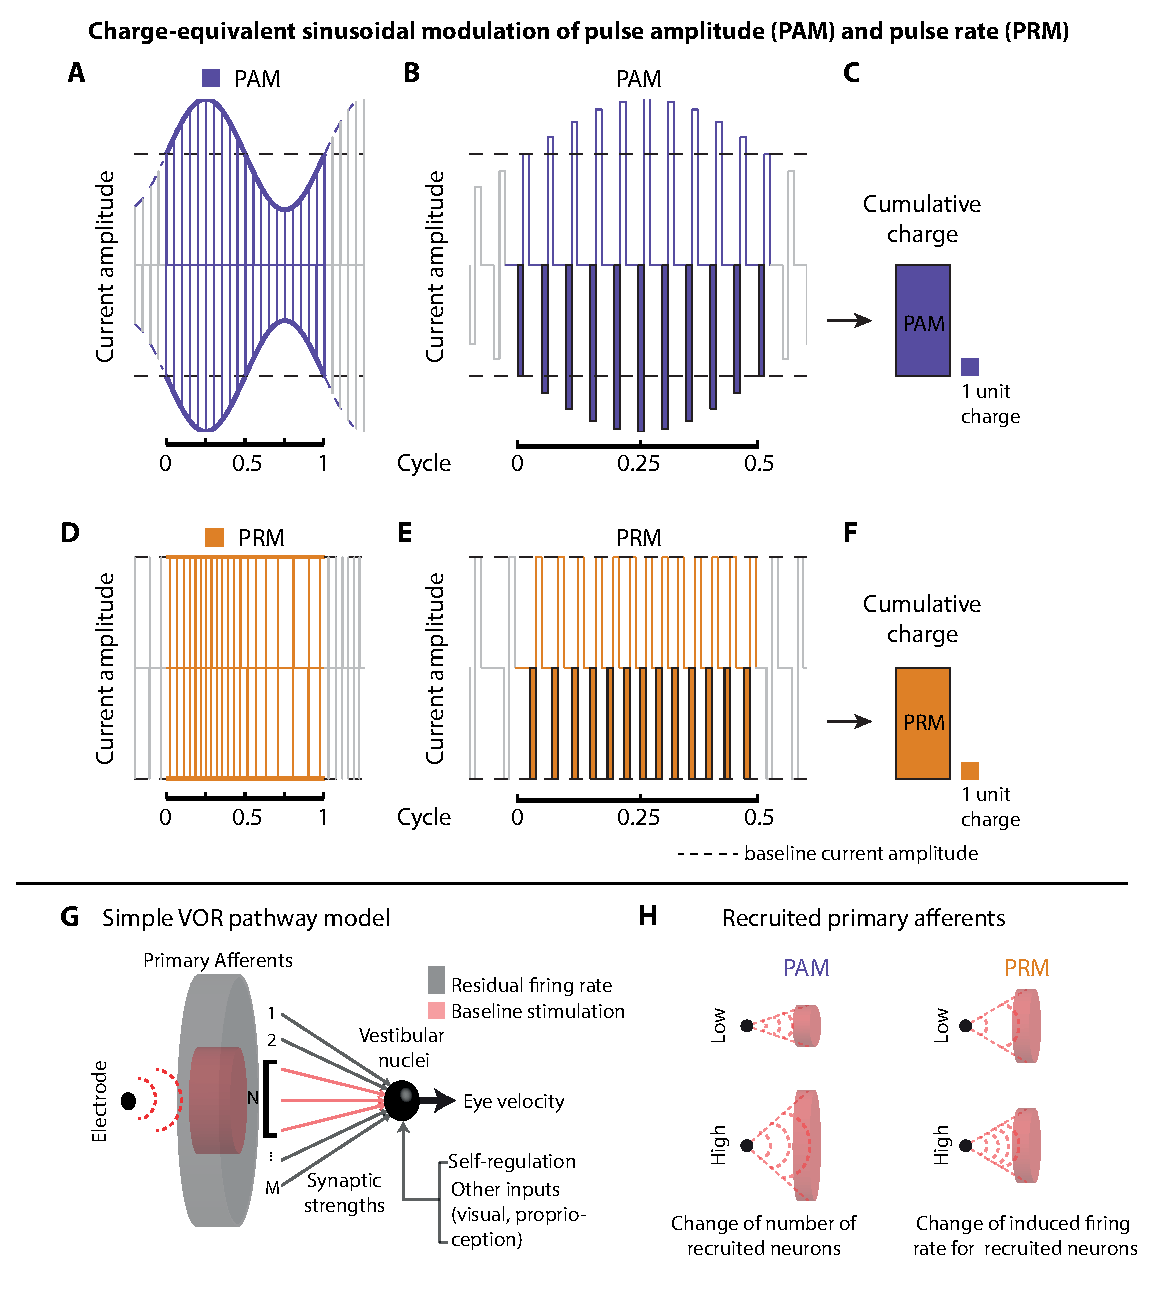
\includegraphics[height=0.63\textheight]{chapters/partii/pamprm/figures/Fig_pamprm_chargemodel.eps} 
\caption[Charge-equivalent PAM, PRM and VOR model]{Visualization of charge-equivalent PAM and PRM, and the VOR pathway model. (\textbf{A}) PAM modulated the pulse amplitude and the intervals between pulses were constant (black dashed lines in plots denote baseline pulse amplitude). (\textbf{B}) Magnification of a half-cycle to illustrate individual pulses during PAM. The injected charge by the cathodic phases (purple areas) during one half-cycle were summed up (\textbf{C}) and PRM parameters were then matched to inject the equivalent charge during (\textbf{D})-(\textbf{F}). Due to symmetry, it sufficed to compute the matched parameter for a half-cycle. Note how the intervals between pulses varied in (D) compared to (A). (\textbf{E}) Within a half-cycle, the PRM paradigm applied thirteen pulses at baseline pulse amplitude, while PAM applied eleven at different current amplitudes. (All plots are not drawn to scale for illustrative purposes.) (\textbf{G}) Illustration of the VOR pathway model. After vestibular injury, afferent neurons continue to fire at some or no resting discharge and are unresponsive to rotational inputs. These afferents synapse directly on the vestibular nuclei; thus have synaptic weights. These weights and any self-regulation must have adapted to equilibrium such that nystagmus is reduced to zero. At the moment the implant is turned on, a discontinuity is introduced. Specifically, there is a sub-population of neurons (red) suddenly firing at baseline pulse rate. We modeled this system as a linear summation (see Appendix). (\textbf{H}) Illustration of the two stimulation paradigms: PAM changes the size of the electric field and thus the number of recruited neurons firing at the baseline pulse rate, whereas PRM does not change the number of recruited neurons, but changes the induced firing rates.}
\label{fig:pamprm:chargemodel}
\end{figure}

\subsection{Vestibular Nuclei Model}
We designed a simple model of the VOR pathway with the vestibular nuclei (VN) (Fig.\,\ref{fig:pamprm:chargemodel}G). The governing equations are listed in the Appendix. Briefly, acute activation of the implant caused a discontinuity that was modeled as a change of firing rate in afferents proximal to the electrode. We simulated 2000 afferents with a lower-than-physiological resting discharge at \SI{30}{\hertz} to emulate vestibular pathology (Fetter and Dichgans, 1996). The VN adapted to implant stimulation by attenuating synaptic weights of recruited afferents and increasing the offset that balanced all afferent input. 
\hyphenation{up-mo-du-lation}
Figure\,\ref{fig:pamprm:chargemodel}H shows afferent recruitment due to prosthetic stimulation. For PAM, increasing sub-populations of afferents were activated during up-modulation, while the inverse occurred during down-modulation. The pulse amplitude determined the radius of the sphere. In contrast, PRM always interacted with the same afferents because pulse amplitude was fixed. These afferents’ firing rates were set by PRM. 

Additionally, we simulated chronic stimulation performance and VOR learning based on retinal slip (Arnold and Robinson, 1997). Conceptually, the model learned from simulated head movement, which were sampled from a distribution reported for walking subjects with vestibular deficiency (Pozzo et al., 1991). The learning rate was identical for PAM and PRM. Similar to acute simulations, synaptic weights were adapted by back-propagation of least-means squares error. Other inputs for learning, such as cerebellum or neighboring brain stem nuclei, were intentionally neglected. We assumed their contributions would be equivalent for PRM or PAM.

\section{Results}
\subsection{Peak Eye Velocities}
Figure\,\ref{fig:pamprm:pev} shows normalized peak eye velocities (PEVs) of the eight electrodes that evoked eye movement responses. Across all patients, PAM resulted in significantly higher responses than PRM at a baseline pulse rate of 200\,pps. 

Modulation levels had no consistent impact (Fig.\,\ref{fig:pamprm:pev}A). High PAM evoked a significantly stronger response than medium PAM in one case (BVL1 SAN). For PRM, a response increase with modulation depth was only observed in BVL3 SAN, a decrease was seen in BVL2 SAN (both non-significant). For other electrodes, modulation levels had a mixed (small) effect on PRM responses. 

BVL3 and BVL4 were additionally tested at a lower 100\,pps baseline pulse rate (Fig.\,\ref{fig:pamprm:pev}B). This led to a significant reduction for PAM, while PRM responses did not change significantly.

\begin{figure}[btp]
\centering
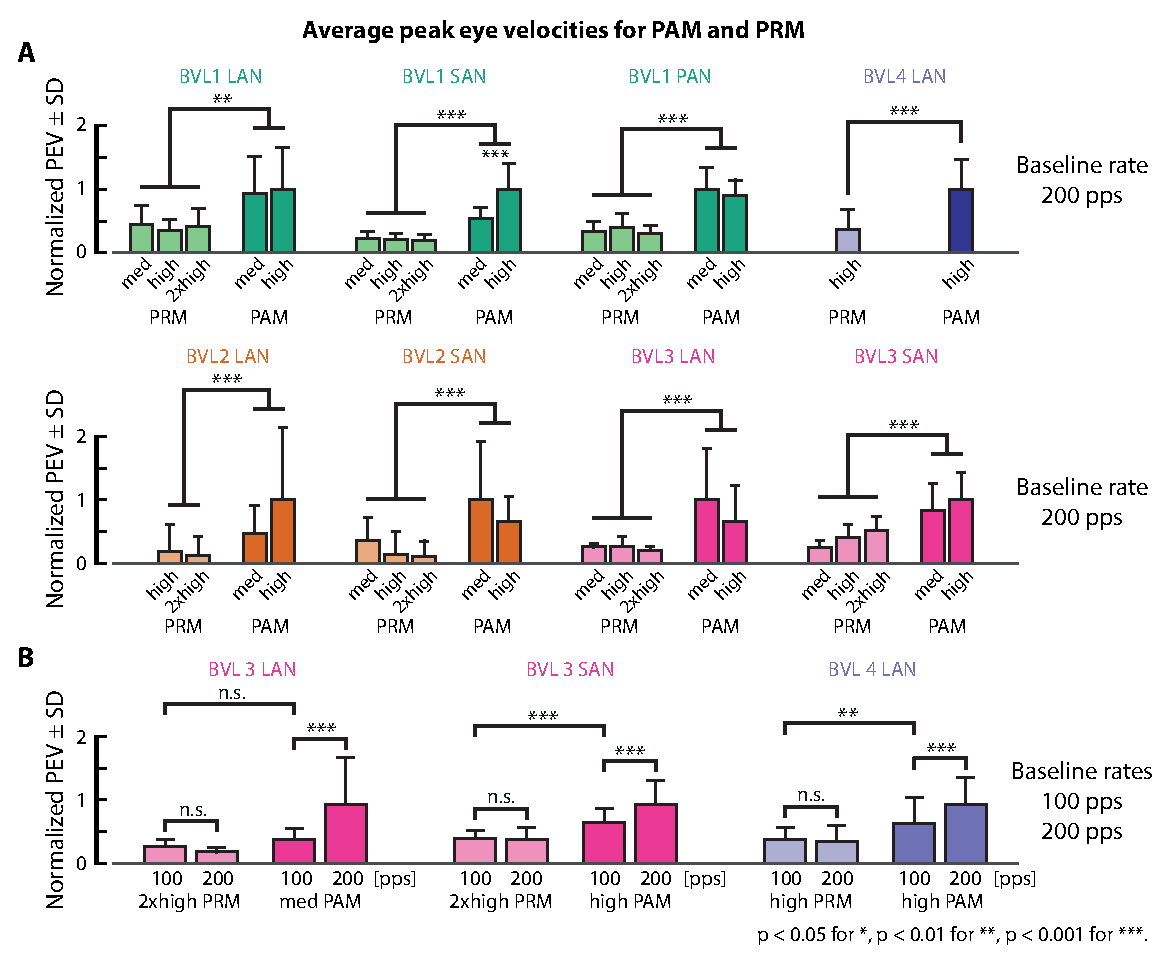
\includegraphics[width=\textwidth]{chapters/partii/pamprm/figures/Fig_pamprm_pev.eps} 
\caption[Average peak eye velocities to PAM and PRM]{Average peak eye velocities (PEV) in response to PAM and PRM. (\textbf{A})-(\textbf{B}) Normalized PEV for different modulation depths at a baseline pulse rate of 200\,pps. Eight out of twelve implanted electrodes evoked eye movement responses. For all electrodes, PAM yielded significantly stronger responses than PRM (p\,\textless\,0.05). Modulation depth did generally not significantly alter PEVs, except for PAM of BVL1 SAN. (Medium PRM for BVL2 LAN is excluded as it failed to show a response significant from zero.) (\textbf{C}) BVL3 and BVL4 were subjected to the lower baseline pulse rate of 100\,pps resulting in reduced PEV for PAM. PRM responses were not significantly changed. For all tests, normalization to the strongest eye movement response, and one-way ANOVA.}
\label{fig:pamprm:pev}
\end{figure}

\subsection{Response Axes}
Figure\,\ref{fig:pamprm:angle}A gives PAM and PRM response axes for LAN electrodes. Activation of these should ideally evoke horizontal eye movement (angle close to 0\degree) and high PRM resulted in response axes closer to 0\degree than high PAM. 

For different modulation levels, PRM response axes did not significantly change (Fig.\,\ref{fig:pamprm:angle}B). For BVL1 and BVL3 LAN, medium to 2xhigh PRM response axes showed a small, non-significant decrease. 

PAM response axes changed significantly with modulation levels for BVL1 and BVL2. Medium PAM axes were closer to 0\degree (improvement of 45\% and 79\%, respectively). 

Halving the baseline pulse rate to 100\,pps moved PAM response axes closer to 0\degree (e.g., 33.2\degree to 10.4\degree for BVL3). PRM response axes did not change for BVL3, whereas for BVL4 a significant increase from 7.8\degree to 21.7\degree was observed.

	For the SAN and PAN electrodes, response axes for PAM and PRM were markedly more vertical (angle closer to 90\degree) than for LAN electrodes (Fig.\,\ref{fig:pamprm:angle}E). Only the axes for BVL3 stayed relatively horizontal (33.5\degree to 44.1\degree). Modulation levels had no significant effect on SAN and PAN response axes. 

\begin{figure}[btp]
\centering
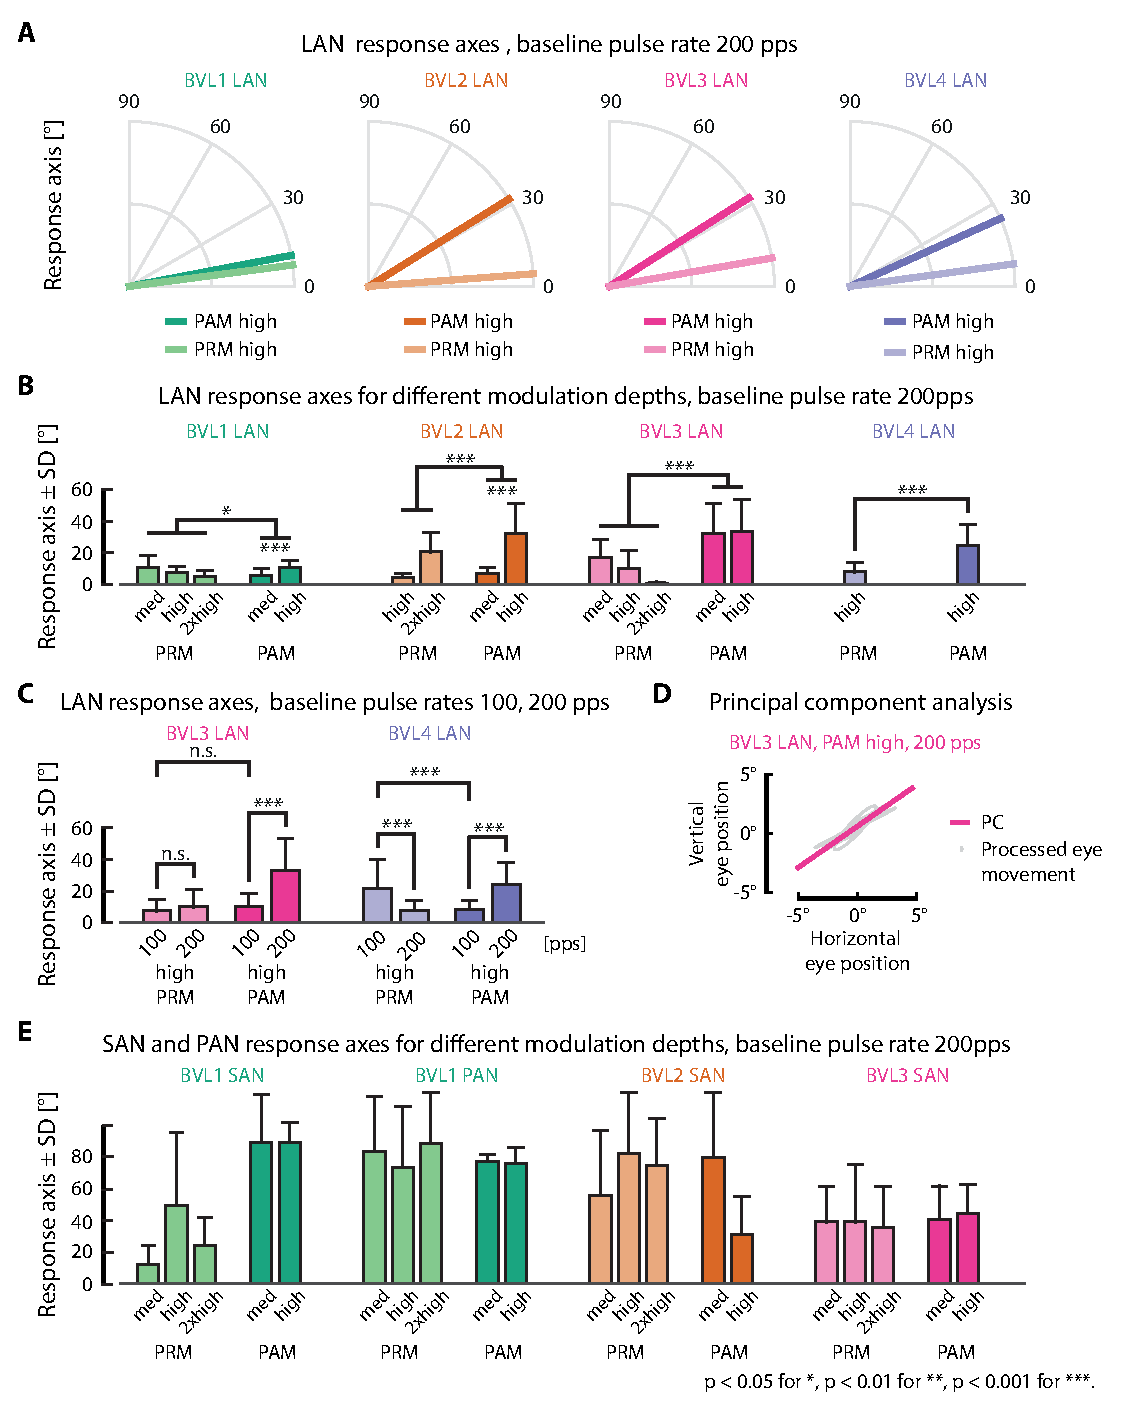
\includegraphics[width=\textwidth]{chapters/partii/pamprm/figures/Fig_pamprm_angle.eps} 
\caption[Eye movement response axes to PAM and PRM]{Eye movement response axes to PAM and PRM with principal component analysis (PCA). (\textbf{A}) Response axes to high level PAM and PRM for the four patients. PRM yielded axes closer to the ideal, horizontal axis in all patients. (\textbf{B}) Modulation depth had a mixed effect on PRM response axes; PAM response axes improved significantly for BVL1 and BVL2. (\textbf{C}) At a lower baseline pulse rate of 100\,pps, PAM yielded responses closer to the horizontal axis than at 200\,pps. PRM response axes were worse than at 200\,pps for BVL4, but not for BVL3. (\textbf{D}) Processed vertical and horizontal eye positions (in grey) for a given modulation were used to calculate the principal component (PC, magenta line), here as an example in BVL3. (\textbf{E}) PAM and PRM response axes for other electrodes. Axes were more vertical than for LAN stimulation as expected. However, a comprehensive comparison was not feasible, since torsional eye movement -- that are also expected with SAN and PAN stimulation -- could not be recorded with our eye tracking system.}
\label{fig:pamprm:angle}
\end{figure}

\subsection{Vestibular Nuclei Model}
First, we simulated the experimental tests at 200\,pps baseline pulse rate of BVL3 LAN (largest absolute PEVs across all electrodes). We found clear differences in the resulting recruitments and ensemble firing rates (Fig.\,\ref{fig:pamprm:model}A-B). This resulted from PAM recruitment being a function of pulse amplitude and the discontinuity between baseline pulse rate and afferent resting discharge. With baseline stimulation, the synaptic weights of recruited afferents decreased compared to non-recruited ones (Fig.\,\ref{fig:pamprm:model}C). Thus action potentials during PAM passed through higher average synaptic weights than PRM. 

	Simulating different modulation levels, PAM generated larger eye movement than PRM (Fig.\,\ref{fig:pamprm:model}D). There were differences within each modality, but the largest change (37.5\%) in pulse rate only generated approximately one-half the eye movement of the smallest change (16.7\%) in pulse amplitude.  
	
	Reducing the baseline pulse rate to 100\,pps changed the adapted synaptic weights and reduced the discontinuity in PAM. As in the experimental results, this caused no change in PEVs for PRM, but reduced PEVs for PAM (Fig.\,\ref{fig:pamprm:model}E).
	
Simulating adaptation to chronic stimulation predicted significantly faster convergence for PAM than PRM (Fig.\,\ref{fig:pamprm:model}F-G). PRM required on average 50\% more steps, but had significantly lower final error. Across head velocities, PRM produced consistently low retinal slip. In contrast, PAM showed large slip for head velocities above 35\,\degree /s, which engaged rarely updated synaptic weights (Fig.\,\ref{fig:pamprm:model}H).

\begin{figure}[btp]
\centering
\includegraphics[height=0.65\textheight]{chapters/partii/pamprm/figures/Fig_pamprm_model-01.eps} 
\caption[Simulations result with vestibular nuclei model]{Simulation results with the vestibular nuclei model. (\textbf{A}) Application of charge-balanced PAM and PRM recruited different afferent sub-populations. (\textbf{B}) Averaging across all afferents, PAM induced a higher ensemble firing rate. (\textbf{C}) After vestibular injury,  synaptic weights were determined by the resting discharge of each afferent. We used a distribution of resting discharge (26.3$\pm$\SI{6.6}{\hertz}); thus the initial weights were also distributed. When the implant was turned on, there was an induced error. (\textbf{D}) Mean eye response to PAM (17 and 25\% modulation) and PRM (17, 25, and 38\% modulation) for 50 cycles; bands are standard deviation. Since experimental PEVs were obtained during increasing pulse amplitude or pulse rate, we focused on the positive model output. (\textbf{E}) Model eye velocity was dependent on baseline pulse rate for PAM. PRM was not affected. (\textbf{F})-(\textbf{H}) Simulation of chronic performance for both stimulation paradigms. (\textbf{F}) Walking was used as an impetus for retinal slip. Both single and mean (n = 100) simulations showed that PAM converged to less than 1\,\degree /s retinal slip significantly faster than PRM (at 200\,pps baseline pulse rate). (\textbf{G}) However, PRM eventually converged to a less variable and significantly lower final value of error. (\textbf{H}) Simulated slips from converged models found that PAM errors were higher for all velocities, especially apparent above 35\,\degree /s. (Bar plots are concatenated from 100 simulations, * is two-sample t-test, p\,\textless\,0.05)}
\label{fig:pamprm:model}
\end{figure}

\section{Discussion}
We acutely tested PAM and PRM in four BVL patients with a VI. Across all responsive electrodes, PAM evoked clearly stronger PEVs than PRM. Although PRM had LAN response axes significantly closer to ideal than PAM, PEVs are more critical since studies have shown that misalignment could be managed. Therefore, PAM should be considered as preferential paradigm for initial VI activation.  

\subsection{Effects of Pulse Modulation on Response Axes}
For LAN stimulation at 200\,pps baseline pulse rate, PRM generally resulted in response axes significantly closer to the ideal horizontal axis than PAM. The size of the electrical field induced by PAM should be modulated, thus possibly recruiting afferents in an adjacent canal, specifically SAN, which presumably would evoke non-horizontal eye movement. Indeed, high PAM in BVL1 and BVL2 had response axes significantly further away from ideal than medium PAM. With PRM, in contrast, the size of the electrical field should remain unchanged and modulation levels did not affect response axes. Our results were in agreement with findings in chinchillas, where PRM response axes were also closer to reference axes than PAM ones (Davidovics et al., 2012).

For a VI to be ultimately useful to patients, it should compensate for all head movements in 3D space. Response axes observed in BVL1 and BVL2 were encouraging in this respect, since LAN and SAN stimulation evoked eye movements predominantly in the horizontal or vertical directions, as expected from physiology. However, some misalignment could be observed. Studies demonstrated that initial misalignment to an ideal axis was significantly reduced over one week of continuous stimulation (Dai et al., 2013). This improvement has been attributed to the plasticity of the vestibular-ocular central nervous system, capable of adapting to activation patterns induced by an implant. Additionally, a coordinate transformation could reduce alignment (Fridman et al., 2010).

\subsection{Effects of Pulse Modulation on Peak Eye Velocity and VN Model}
In VIs for animal models, PRM has often been selected as encoding scheme to mimic the primary vestibular afferents’ spike rate modulation (Merfeld and Lewis, 2012). However, PAM also elicited viable eye movement responses in patients (Guyot et al., 2011b) and has recently become more relevant as stimulation paradigm with the more widespread adoption of modified cochlear implants for vestibular stimulation (Valentin et al., 2013; Golub et al., 2014; Perez Fornos et al., 2014). Our findings revealed PAM’s capability to evoke strong eye movements. Furthermore, they demonstrated that PAM was more charge-efficient than PRM, potentially extending battery life. 

	Modulation levels had generally no effect on PAM PEVs, most likely due to small increments between medium and high PAM in our subjects (modulation depths less than 30\%). PEVs significantly increased with modulation depth only for BVL1 SAN for unknown reasons. These differences in PEVs across electrodes highlight the need for a better understanding of the underlying subject-specific pathologies to potentially adjust electrode design, electrode placement and to optimize modulation range. The insensitivity of PRM PEVs for different modulation levels, even at 2xhigh, may be due to the high baseline pulse rate.
	
For baseline pulse rates 100 and 200\,pps, PEVs to PRM were practically identical, while PAM elicited stronger responses at the higher baseline pulse rate. A similar effect with higher baseline pulse rates favoring PAM was reported in chinchillas (Davidovics et al., 2012) and rhesus monkeys (Davidovics et al., 2013). 

The VN model revealed the different efficacies for charge-balanced PRM and PAM. First, PAM recruited additional sub-populations of afferents and triggered a sharp change in firing rates from resting discharge to the higher, induced pulse rate. Second, these sub-populations had greater synaptic weights, as they were not attenuated by adaptation to baseline stimulation. Engaging these weights, therefore, led to significantly larger PEVs with PAM than with PRM. In contrast, PRM was confined to the same sub-population with attenuated weights and had no access to sub-populations with greater weights. These mechanisms also revealed that PAM was strongly dependent on the baseline pulse rate, while PRM had minimal dependency, as found in our experiments. 

Chronic stimulation in patients was not approved at the time of this study. Evidence from animal research suggests that chronic stimulation could improve responses. Chronic PRM responses improved significantly during continuous stimulation (90 days) at baseline pulse rates above 200 pps, likely due to VOR learning (Lewis et al., 2010). To our knowledge chronic PAM studies in animal models have not been reported. It is therefore possible that PAM responses could improve chronically, too.

The VN model also simulated chronic stimulation and adaptation. These simulations highlighted effects of PRM and PAM engaging different afferent populations. PAM generated larger PEVs and thus larger retinal errors, which facilitated learning. However, this learning was inconsistent as synaptic weights for rarely sampled high head velocities were updated rarely (Fig.\,\ref{fig:pamprm:model}H). In contrast, PRM continuously updated the same synaptic weights and learned a lower error solution across all head velocities.

\section{Summary}
Our experimental findings and model simulations strongly support PAM at 200\,pps baseline pulse rate as preferential acute stimulation paradigm. The findings add urgency to investigate chronic stimulation with PAM, as its chronic efficacy remains an open issue. 

\begin{landscape}
\section*{Appendix -- Subject Details}
\markright{Appendix -- Subject Details}
\addcontentsline{toc}{section}{Appendices}

\begin{table}[h]\tiny
\centering
\caption[Patient demographics and stimulation parameters]{\footnotesize Patient demographics and stimulation parameters. Cursive printed modulation depths denote setting for largest eye movement response for corresponding electrode.}\label{tab:pamprm}
\begin{tabularx}{\linewidth}{YYYYYYYYYY}
\toprule
Patient & Sex, etiology & Age at implantation, implanted ear & Electrode & Baseline pulse rate [pps] & Baseline pulse amplitude [\SI{}{\micro\ampere}] & Level & PAM [$\pm$\SI{}{\micro\ampere}], (modulation depth) & PRM [$\pm$pps], (modulation depth) & Largest electrode response [\degree /s]\\
\midrule
{\multirow{9}{*}{BVL1}} & {\multirow{9}{*}{Male, DFNA9}}& {\multirow{9}{*}{66,left}} & {\multirow{3}{*}{LAN}}& {\multirow{3}{*}{200}} & {\multirow{3}{*}{200}} & medium & 15 (7.5\%) & 10 (5\%) &{\multirow{3}{*}{1.8}}\\
& & & & & & high & \textit{25 (12.5\%)} & 20 (10\%)\\
& & & & & & 2xhigh & & 40 (20\%) \\ \cline{4-10}
& & & {\multirow{3}{*}{SAN}}& {\multirow{3}{*}{200}} & {\multirow{3}{*}{155}} & medium & 15 (9.7\%) & 22 (11\%) &{\multirow{3}{*}{4.9}}\\
& & & & & & high & \textit{25 (16.1\%)} & 29 (14.5\%) \\
& & & & & & 2xhigh & & 56 (28\%)\\ \cline{4-10}
& & & {\multirow{3}{*}{PAN}}& {\multirow{3}{*}{200}} & {\multirow{3}{*}{200}} & medium & \textit{38 (19\%)} & 37 (18.5\%) &{\multirow{3}{*}{3.6}}\\
& & & & & & high & 56 (28\%) & 55 (27.5)\\
& & & & & & 2xhigh & & 112 (56\%)\\ \cline{1-10}

{\multirow{9}{*}{BVL2}} & {\multirow{9}{*}{Female, DFNA9}}& {\multirow{9}{*}{68,left}} & {\multirow{3}{*}{LAN}}& {\multirow{3}{*}{200}} & {\multirow{3}{*}{300}} & medium & 25 (8.3\%) & 16 (8\%), no response &{\multirow{3}{*}{1.4}}\\
& & & & & & high & \textit{50 (16.7\%)} & 34 (17\%)\\
& & & & & & 2xhigh & & 50 (25\%) \\ \cline{4-10}
& & & {\multirow{3}{*}{SAN}}& {\multirow{3}{*}{200}} & {\multirow{3}{*}{350}} & medium & \textit{34 (9.7\%)} & 18 (9\%) &{\multirow{3}{*}{1.2}}\\
& & & & & & high & 50 (14.3\%) & 27 (13.5\%) \\
& & & & & & 2xhigh & & 84 (42\%)\\ \cline{1-10}
\end{tabularx}
\end{table}
\pagebreak
\begin{table}[h]\tiny
\centering
\begin{tabularx}{\linewidth}{YYYYYYYYYY}
\toprule
Patient & Sex, etiology & Age at implantation, implanted ear & Electrode & Baseline pulse rate [pps] & Baseline pulse amplitude [\SI{}{\micro\ampere}] & Level & PAM [$\pm$\SI{}{\micro\ampere}], (modulation depth) & PRM [$\pm$pps], (modulation depth) & Largest electrode response [\degree /s]\\
\midrule
{\multirow{12}{*}{BVL3}} & {\multirow{12}{*}{Female, trauma}}& {\multirow{12}{*}{67,left}} & {\multirow{3}{*}{LAN}}& {\multirow{3}{*}{200}} & {\multirow{3}{*}{300}} & medium & \textit{50 (16.7\%)} & 34 (17\%) & {\multirow{3}{*}{7.8}}\\
& & & & & & high & 75 (25\%) & 50 (25\%)\\
& & & & & & 2xhigh & & 75 (37.5\%) \\ \cline{4-10}
& & & {\multirow{3}{*}{LAN}} & {\multirow{3}{*}{100}} & {\multirow{3}{*}{300}} & medium & \textit{50 (16.7\%)} &  &{\multirow{3}{*}{1.2}}\\
& & & & & & high & 75 (25\%) & 36 (36\%) \\
& & & & & & 2xhigh & & 72 (72\%)\\ \cline{4-10}
& & & {\multirow{3}{*}{SAN}}& {\multirow{3}{*}{200}} & {\multirow{3}{*}{400}} & medium & 50 (12.5\%) & 26 (13\%) & {\multirow{3}{*}{4.0}}\\
& & & & & & high & \textit{75 (18.8\%)} & 39 (19.5\%)\\
& & & & & & 2xhigh & & 80 (40\%) \\ \cline{4-10}
& & & {\multirow{3}{*}{SAN}}& {\multirow{3}{*}{100}} & {\multirow{3}{*}{350}} & medium & 50 (14.3\%) &  &{\multirow{3}{*}{1.2}}\\
& & & & & & high & \textit{100 (28.6\%)} & 27 (27\%) \\
& & & & & & 2xhigh & & 54 (54\%)\\ \cline{1-10}

{\multirow{2}{*}{BVL4}} & {\multirow{2}{*}{Male, DFNA9}}& {\multirow{2}{*}{66,left}} & {\multirow{1}{*}{LAN}}& {\multirow{1}{*}{200}} & {\multirow{1}{*}{120}} & medium & \textit{60 (50\%)} & 100 (50\%) & {\multirow{1}{*}{7.6}}\\ \cline{4-10}
& & & {\multirow{1}{*}{LAN}}& {\multirow{1}{*}{100}} & {\multirow{1}{*}{120}} & medium & \textit{60 (50\%)} & 50 (50\%) & {\multirow{1}{*}{2.8}}\\

\bottomrule 
\end{tabularx}
\end{table}
\end{landscape}
\section*{Appendix -- Vestibular Nuclei Model Equations}
\markright{Appendix -- Vestibular Nuclei Model Equations}
\begin{itemize}
\item Model specification, i.\,e. before stimulation onset
\begin{align*}
v &= \tanh \left( \sum_N w_i x_i + b \right) = 0 \\
\intertext{\item Output at VI activation, baseline stimulation}
v & = \tanh \left( \sum_N w_i {\color{red}{x_i}} + b \right) \neq 0\\
\intertext{\item Adaptation to minimize nystagmus}
\epsilon &= 0 - v\\
\delta w_i &= \alpha_w e\left(1.1 - v^2 \right) x_i\\
\delta b &= \alpha_{\text{bias}} e \left( 1.1 - v^2\right)
\end{align*}
\end{itemize}
where $v$ is peak eye velocity output, $N$ the total number of afferents, $w_i$ their synaptic weights, $x_i$ the afferents' spontaneous or induced firing rate, $b$ the bias term. Before stimulation onset, at rest, afferents are firing at their spontaneous resting discharge rate and $v$ is zero. The $\tanh$ function introduces a linear and saturated regions that replicate natural behavior. 

When baseline stimulation is activated, a number of afferents is recruited by the stimulation and their firing rate $x_i$ will change. This results in eye movement that contradicts the stationary visual surrounding (subject sitting in a chair). The resulting error $e$ is minimized to zero through adaptation of synaptic weights and the learning rates $\alpha_w$, $\alpha_{\text{bias}}$ for the afferents and bias, respectively.